
\chapter{Perspectives\label{chpt:perspectives}}

A great deal of unfinished work and theories linked to this thesis
is presented here.Polarizable and/or flexible models of solute, and
the coupling of a QM solute to the molecular solvent, will be described
in perspective.

\section{Reduce memory use in MDFT}

The total CPU time to implement a MDFT minimization using \texttt{\textbf{convolution}}
algorithms is typically 1 to 30 minutes according to the resolution
of grid. But the memory consumed for such a process is typically 1
to 20 G of RAM. This is mainly due to the minimizer L-BFGS-B, which
firstly needs to store several steps of information during the iterations,
and secondly it is in double precision, it is to say that the density
variable $\rho(\mathbf{r},\mathbf{\Omega})$ and the gradient also
need to be stored in double precision, if not, as tested, it leads
to a divergence of result. In addition, during the evaluation of functional,
memory at most 3 times of $\rho(\mathbf{r},\mathbf{\Omega})$ needs
to be stored simultaneously.

There are to ways to get over this memory limit, and both of them
need to modify the L-BFGS-B minimizer, which is a ``blackbox'',
in Fortran 77. 

The simplest way is to change the double precision to float number
of the L-BFGS-B minimizer, this action can reduce the memory needed
by 2. 

And another way to completely pass this limit, is to parallelize is
code to several nodes using MPI. This requires only to modify the
\acs{FFT} and L-BFGS-B process, where their is a mixing of variables
$\rho(\mathbf{r},\mathbf{\Omega})$.

\section{Site-site grid}

The \acs{IET} uses intermolecular spherical coordinates, and cannot
describe huge molecules. \acs{MDFT} uses a homogeneous spatial grid,
thus have the same resolution near and far from the solute. To meet
a satisfying result, sometimes a finer resolution is needed. Another
natural way to think about construction of the grid is like in \ref{fig:Site-site-grid-model},
an spherical grid at each site of solute. 

\begin{figure}[h]
\begin{centering}
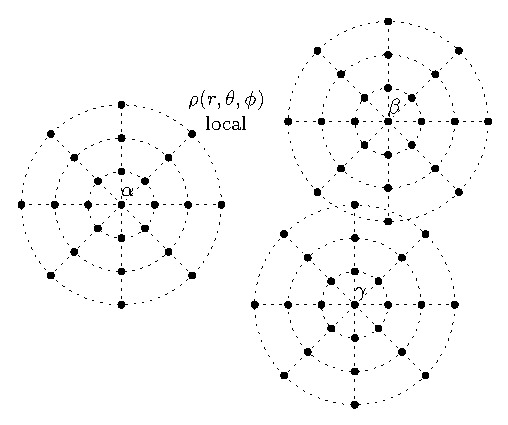
\includegraphics{_figure/site-site}
\par\end{centering}
\caption{Site-site grid model\label{fig:Site-site-grid-model}}
\end{figure}

The idea can be roughly understand as an interaction site treatment
of the solute, with a molecular treatment of the solvent. It is a
matrix of $h_{\text{MS}}(1,2)$ with a full molecular description
of $c_{\text{SS}}(1,2)$. As in \acs{MDFT} the solvent density can
be else than particle-particle distribution functions, it is possible
to have different descriptions for solute and solvent. The formalism
is possible, also as the e\acs{DFT} shares some formalism with c\acs{DFT},
a site description of solute which is used as default in \acs{QM}
calculations should also gives some inspiration to the liquid theory.
(Or I think it is like 3D-RISM, but their is no correspondent \acs{DFT}
theory, nor basis set description of site.) If the sites are expanded
onto spherical harmonics $Y_{lm}$, there is also a rotational invariance
between the sites, and the inhomogeneous angular grid can be thus
ignored, it is only an issue of $\mathbf{r}_{\text{M}}-\mathbf{r}_{\text{N}}$
between site M and N. This is only an idea, the mathematical deduction
is not yet fully verified.

The generalized \acs{OZ} equation to $n$ components
\begin{equation}
h_{\nu\mu}(1,2)=c_{\nu\mu}(1,2)+\rho\sum_{\lambda}x_{\lambda}\int c_{\nu\lambda}(2,3)h_{\lambda\mu}(1,3)\mathrm{d}3
\end{equation}
thus
\begin{equation}
h_{\text{MS}}(1,2)=c_{\text{MS}}(1,2)+\rho\int c_{\text{SS}}(2,3)h_{\text{MS}}(1,3)\mathrm{d}3
\end{equation}
\begin{equation}
h_{\text{NS}}(1,2)=c_{\text{NS}}(1,2)+\rho\int c_{\text{SS}}(2,3)h_{\text{NS}}(1,3)\mathrm{d}3
\end{equation}
Look that $c_{\text{SS}}(2,3)$ is just the bulk \acs{DCF}. The link
between $h_{\text{MS}}(1,2)$ and $h_{\text{NS}}(1,2)$ is a translation
of center $\mathbf{r}_{\text{M}}-\mathbf{r}_{\text{N}}$\textcolor{red}{(?)}.
Therefore, ...

\section{Polarizable solute, other improvement of the external term}

During the iteration, the $V_{\mathrm{ext}}$ is fixed. It can be
a variable by adding an extra variable term linked to the dipole of
solute $\mu_{M}$, such that this part can be calculated for each
iteration, and can be minimized.

\section{MDFT Viewer}

This thesis contains originally a segment on visualization. Due to
time limit, it is removed. Viewer is an important part of code development,
which provides beautiful visualization and easy analysis, and helps
to popularize the code. GaussViewer is a good example.

The popular language of visualization is c++, OpenDM, ...

The process of MDFT can produce energy and structures for each iteration,
although it takes time to write down all the possible output.

\section{Application to real biological systems}

Reinvestigation of the Manganese-oxo 

This is the case we talked about in the introduction, ...
